\documentclass[a5paper]{article}
\usepackage[a5paper, top=8mm, bottom=8mm, left=8mm, right=8mm]{geometry}

\usepackage{polyglossia}
\setdefaultlanguage[babelshorthands=true]{russian}

\usepackage{fontspec}
\setmainfont{FreeSerif}
\newfontfamily{\russianfonttt}[Scale=0.7]{DejaVuSansMono}

\usepackage[font=scriptsize]{caption}

\usepackage{amsmath}
\usepackage{amssymb,amsfonts,textcomp}
\usepackage{color}
\usepackage{array}
\usepackage{hhline}
\usepackage{cite}
\usepackage{textcomp}

\usepackage[hang,multiple]{footmisc}
\renewcommand{\footnotelayout}{\raggedright}

\PassOptionsToPackage{hyphens}{url}\usepackage[xetex,linktocpage=true,plainpages=false,pdfpagelabels=false]{hyperref}
\hypersetup{colorlinks=true, linkcolor=blue, citecolor=blue, filecolor=blue, urlcolor=blue, pdftitle=1, pdfauthor=, pdfsubject=, pdfkeywords=}

\newlength\Colsep
\setlength\Colsep{10pt}

\usepackage{tabu}

\usepackage{graphicx}
\usepackage{indentfirst}
\usepackage{multirow}
\usepackage{subfig}
\usepackage{footnote}
\usepackage{minted}

\newcommand{\todo}[1] {
\begin{center}\textcolor{red}{TODO: #1}\end{center}
}

\newcommand{\attribution}[1] {
    \vspace{-5mm}\begin{flushright}\begin{scriptsize}%\textcolor{gray}
    {\textcopyright\, #1}\end{scriptsize}\end{flushright}
}

\sloppy
\pagestyle{plain}

\title{Лекция 6: Структурные шаблоны}
\author{Юрий Литвинов\\\small{yurii.litvinov@gmail.com}}
\date{}

\begin{document}

\maketitle
\thispagestyle{empty}

\section{Введение}

\subsection{Зачем паттерны и зачем их изучать?}

Шаблоны (или паттерны) проектирования --- это набор стандартных решений, применяемых в типичных ситуациях. Популяризованы они были в середине 90-х годов знаменитой книгой <<Приёмы объектно-ориентированного проектирования. Паттерны проектирования>> Э. Гамма, Р. Хелм, Р. Джонсон, Д. Влиссидес (так называемая <<банда четырёх>>, известные популяризаторы объектно-ориентированного программирования). В академической среде про паттерны начали говорить ещё раньше (и вообще, всё пошло из городской архитектуры, К. Александера <<Язык шаблонов. Города. Здания. Строительство>> 1977 года), но по-настоящему актуальны они стали в связи со взрывным развитием объектно-ориентированных языков в 90-х и появлением Java (хотя первое издание книги использовало язык Smalltalk). В конце 90-х и в 2000-х на паттерны чуть ли не молились, вышло несколько переизданий оригинальной книги и десятки других книг, курсов и сайтов с красивыми картинками, что хорошая новость, потому что найти материал для подготовки по этой теме ничего не стоит (и я бы даже рекомендовал не читать этот конспект, а найти на просторах интернета что-нибудь, что вам больше понравится --- современное издание книги <<банды четырёх>> вполне подойдёт, можно и что-то другое, но что-то про паттерны прочитать точно надо). 

Сейчас, тем не менее, сообщество сходится на том, что паттерны проектирования предназначены скорее для борьбы с недостатками Java и для современных языков не так актуальны. И действительно, с 90-х годов языки (даже консервативная Java) успели эволюционировать, некоторые паттерны оказались встроенными в язык (например, паттерн <<Наблюдатель>> реализован в C\# с помощью механизма событий), некоторые оказались больше не так полезны (например, повсеместное использование лямбда-функций делает паттерн <<Стратегия>> несколько избыточным). Кроме того, можно сказать, что популярные языки программирования постепенно смещаются в сторону функциональной парадигмы, а она паттерны проектирования вообще отрицает (хотя функциональные паттерны тоже, конечно, есть --- например, Continuation Passing Style и монады, это, по сути, паттерны). Тем не менее, паттерны проектирования до сих пор считается приличным знать любому адекватному программисту, про них практически всегда спрашивают на собеседованиях, так что в этом курсе на паттерны проектирования отводится аж три лекции. На самом деле, знать паттерны полезно даже если ими не пользоваться --- они очень хорошо открывают глаза на объектно--ориентированное программирование и <<тактическую>> архитектуру, показывают ряд интересных приёмов.

\subsection{Что такое паттерны}

Итак, следуя Википедии, \textit{паттерн проектирования} --- это повторяемая архитектурная конструкция, представляющая собой решение проблемы проектирования в рамках некоторого часто возникающего контекста\footnote{Шаблон проектирования, URL: \url{https://ru.wikipedia.org/wiki/Шаблон_проектирования}}. Паттерны

\begin{itemize}
    \item имеют имя, что позволяет унифицировать терминологию и упростить общение между разработчиками --- гораздо проще сказать <<Тут реализован паттерн ``Состояние''>>, чем долго объяснять, как он работает;
    \item широко известны, так что если вы говорите <<Тут реализован паттерн ``Состояние''>>, можно смело рассчитывать, что вас поймут;
    \item изложены структурированно и в удобной для изучения форме, что помогает переиспользованию знаний и быстрому введению молодых специалистов в суть дела;
    \item подходят для решения целого класса проблем, которые возникают в разных предметных областях при программировании на разных языках --- так что они достаточно универсальны, чтобы их стоило изучать на общем курсе по архитектуре.
\end{itemize}

При этом паттерны не:

\begin{itemize}
    \item не конкретный рецепт или указания к действию --- паттерны скорее стоит понимать как идеи или красивые приёмы, которые можно использовать или от которых можно отталкиваться при проектировании;
    \item не приёмы использования конкретных языков --- бывают языковые идиомы, например, RAII\footnote{Resource Acquisition Is Initialization, идиома, связывающая управляемые ресурсы типа открытых файлов или сетевых соединений с временем жизни объекта, который их представляет в программе} в C++, это не паттерны. Паттерны должны быть применимы в рамках целой парадигмы программирования, вне зависимости от языка.
\end{itemize}

Начинающие проектировщики часто понимают паттерны именно как конкретные рецепты или даже как просто что-то хорошее, что делает любую архитектуру лучше --- в своё время был популярен анекдот про то, как кто-то написал Гамме письмо, что он уже использовал в своём проекте 12 паттернов из книжки, и может ли ему Гамма подсказать, куда вставить оставшиеся. Это очень неправильная точка зрения, паттерн --- это именно идея, хорошо зарекомендовавшая себя в некоторых распространённых ситуациях. Идею можно по-разному реализовать, можно модифицировать, и часто описания паттернов включают в себя рассуждения по поводу разных вариантов. Так что бояться отклониться от шаблона не надо --- единственное, что в рамках этого курса всё-таки стоит научиться делать как положено, а уже потом, как паттерны будут освоены, менять их и подстраивать под конкретные ситуации.

Паттерны условно делятся на \textit{структурные}, \textit{поведенческие} и \textit{порождающие}. Структурные паттерны по идее описывают особенности структуры во время компиляции, поведенческие занимаются поведением системы во время выполнения, а порождающие описывают разные способы создавать сложные группы объектов. Однако разделение это очень условно, поэтому мы не будем его строго придерживаться, и не рекомендую пытаться запомнить, какой паттерн к какой группе относится: например, в книге <<Банды Четырёх>> паттерн <<Декоратор>> относится к структурным, а паттерн <<Стратегия>> к поведенческим, хотя они очень похожи по смыслу. Тем не менее, в литературе такое разделение встречается часто.

\subsection{Место паттернов в архитектуре}

В одной из презентаций проф. N. Medvidovic из USC была картинка, проясняющая место паттернов проектирования в архитектуре, она воспроизведена на рис~\ref{image:patterns}.

\begin{figure}
    \begin{center}
        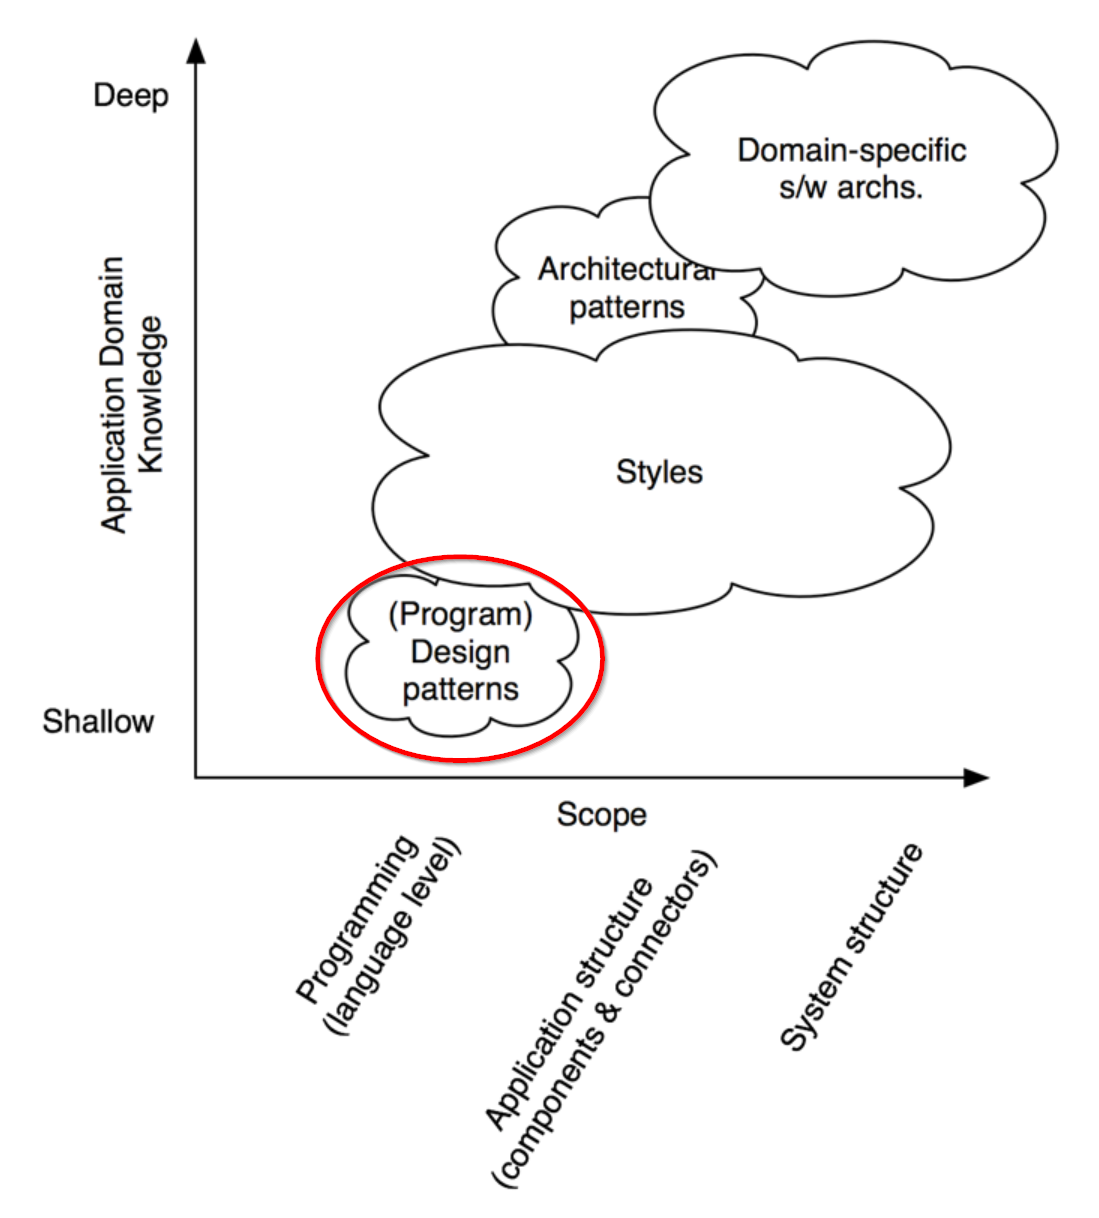
\includegraphics[width=0.55\textwidth]{architecturalStylesPatternsHighlighted.png}
    \end{center}
    \caption{Место паттернов проектирования в архитектуре.}
    \label{image:patterns}
\end{figure}

Паттерны проектирования не специфичны для предметной области и могут успешно применяться в самых разных контекстах, вместе с тем они предлагают тактические архитектурные решения, не затрагивая общую архитектуру приложения или подсистемы. Поэтому паттерны проектирования занимают левую нижнюю часть картинки. На самом деле, паттерны проектирования можно понимать как границу между программированием и архитектурой --- если вы детализировали архитектуру до уровня, что понятно, какие паттерны где применять, стоит остановиться и большую детализацию отложить на этап реализации. Если в команде есть выделенный архитектор, то использование паттернов ему ещё может быть интересно, а вот как именно они реализуются --- он может доверить программистам.

В этом курсе мы начнём с паттернов и поговорим также и про архитектурные стили и (немного) про архитектурные паттерны. А вот про предметно-ориентированные архитектуры говорить не будем, потому что они актуальны только в рамках конкретной предметной области --- например, существуют референсные архитектуры для автомобильного или аэрокосмического программного обеспечения, они очень подробно описывают структуру приложений, протоколы коммуникации и т.п., и следование им обязательно для успешной сертификации (которая в большинстве случаев обязательна в этих областях). Поскольку вероятность того, что кто-то из слушателей этого курса столкнётся с какой-то конкретной референсной архитектурой, минимальна (и поскольку каждая из них заслуживает отдельного курса), мы их обсуждать не будем.

\subsection{Модельный пример}

Дальше мы перейдём наконец к конкретным паттернам. Изложение в большинстве случаев будет, следуя книге <<банды четырёх>>, вестись на примере текстового редактора. Положим, мы хотим разработать свой текстовый редактор с нуля, причём это должен быть WYSIWYG\footnote{What You See Is What You Get}-редактор --- редактор, где страница при редактировании выглядит так, как она будет напечатана или сохранена (наподобие Microsoft Word и в противоположность TeX, где редактируется специальная разметка, а для получения результата требуется компиляция). Для того, чтобы написать такой редактор, нам потребуется решить ряд архитектурных вопросов.

\begin{itemize}
    \item Как представляется внутри редактора структура документа? Документ ведь надо не только выводить на экран, но и эффективно хранить в памяти, так, чтобы эффективно выполнять разные операции (типа редактирования, форматирования и т.д.).
    \item Как будет работать форматирование документа, в смысле размещение текста на странице, выравнивание и т.д.? Поскольку у нас WYSIWYG-редактор, нам важна скорость работы, но также важно и качество результата, так что, как и всегда, имеются конфликтующие требования.
    \item Как мы реализуем красивый и удобный интерфейс пользователя? Поскольку у нас курс по архитектуре, вопросы типа размещения и цвета кнопок нас не волнуют, но нам надо придумать архитектуру такой, чтобы дизайнер мог легко воплотить самые разные свои идеи.
    \item Как поддержать разные стандарты внешнего облика программы? В разных операционных системах look and feel программы по традиции свой, хочется безболезненно приспосабливаться под разные стандарты.
    \item Как поддержать команды, которые пользователь может выполнять с редактором, операции отмены и повторения команд? Кажется, что проблема мелкая, но если о ней заранее не подумать, встроить поддержку undo/redo в готовый редактор может оказаться очень сложно --- реализовать для каждой из десятков операций undo/redo отдельно можно с ума сойти.
    \item Как будут выполняться разные аналитические операции типа проверки правописания и расстановки переносов? Сами операции могут быть весьма нетривиальны, не хочется их реализовывать в одной общей куче кода.
\end{itemize}

\section{Паттерн <<Компоновщик>>}

\subsection{Мотивирующий пример}

Начнём рассмотрение паттерна <<Компоновщик>> с мотивирующего примера, и попытаемся придумать ответ на первый вопрос из списка выше --- как представлять внутреннюю структуру документа? Документ по сути --- это множество графических элементов: букв, изображений (буквы по сути сами изображения, так что разница между ними с точки зрения внутреннего представления довольно условна), составных объектов: разных таблиц, колонок и т.п. Строка и страница тоже могут рассматриваться как составные объекты, и составные объекты могут содержать другие объекты --- таблица может состоять из ячеек, содержащих строки, в которых содержатся символы и изображения. Таким образом, наверное, внутреннее представление документа древовидно.

При этом нам надо предоставить пользовательскому интерфейсу способ легко манипулировать внутренним представлением документа. В частности, кроме очевидных операций вставки и удаления элементов в документ, надо уметь:

\begin{itemize}
    \item эффективно генерировать по документу его визуальное представление;
    \item уметь эффективно находить по координатам на экране элемент во внутреннем представлении --- например, кликнули по документу и надо понять, какой элемент документа будет выделен.
\end{itemize}

С точки зрения архитектурной красоты нам также хочется, чтобы текст, графика и составные объекты хранились и обрабатывались единообразно, чтобы разные операции, которым не надо знать подробностей об элементе, могли их не знать. Например, операции форматирования, по сути, надо знать только размеры элементов, чтобы она могла их разместить на странице. Операции отрисовки надо, чтобы элемент мог сообщить свои координаты, размер и что надо нарисовать --- ей не важно, буква это, изображение или вообще таблица или математическая формула.

Поэтому мы приходим к древовидной структуре, называемой в книге банды четырёх <<рекурсивная композиция>>:

\begin{center}
    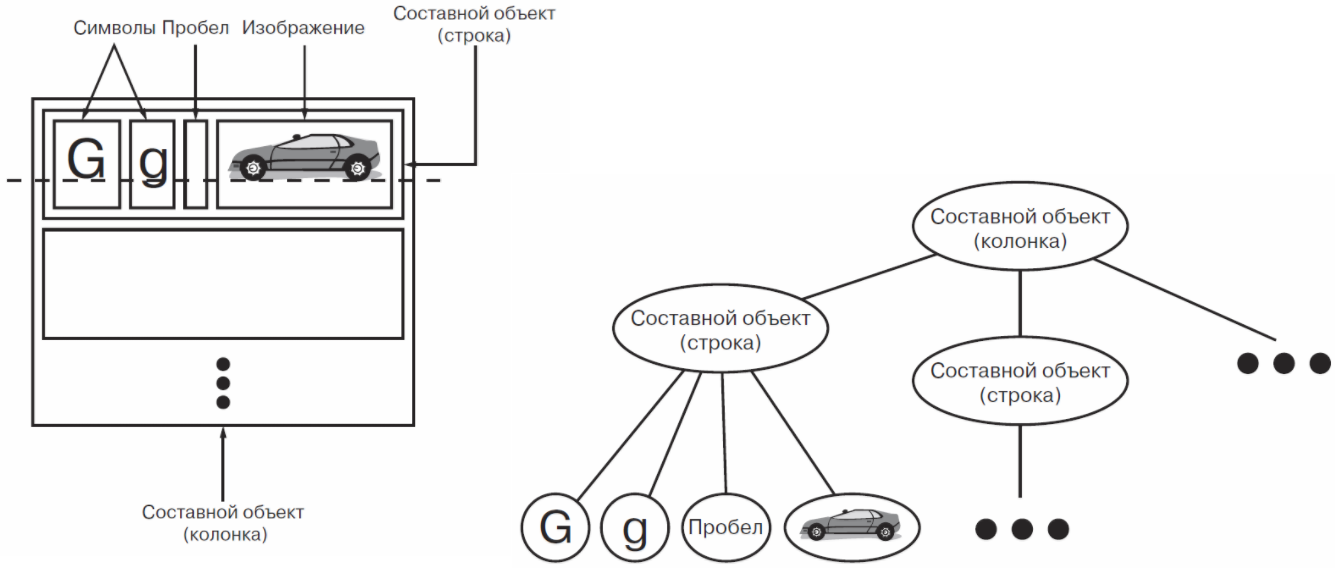
\includegraphics[width=0.9\textwidth]{recursiveComposition.png}
    \attribution{Э. Гамма и др., Приемы объектно-ориентированного проектирования}
\end{center}

То есть любой документ представляется как дерево, где листья --- это элементарные составляющие документа, которые никакой внутренней структуры уже не умеют (буквы, изображения), а внутренние узлы могут быть разными составными объектами (строка, колонка). С точки зрения диаграммы классов эта структура выглядит как-то так:

\begin{center}
    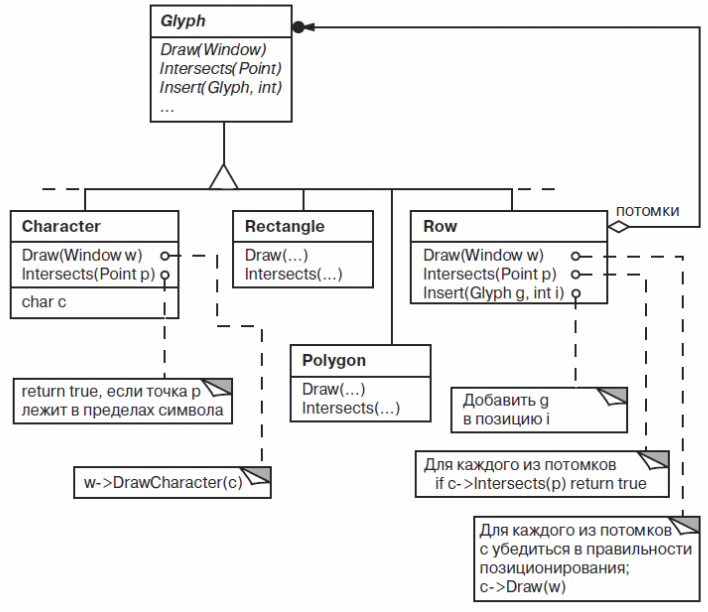
\includegraphics[width=0.7\textwidth]{glyphs.png}
    \attribution{Э. Гамма и др., Приемы объектно-ориентированного проектирования}
\end{center}

Чтобы элементы можно было вкладывать друг в друга, им требуется общий базовый класс (у нас это Glyph, <<Глиф>> --- всё, что может быть нарисовано). В базовом классе определяются операции операции, нужные основной функциональности редактора --- отрисовка, определение принадлежности точки глифу (это для того, чтобы понять, на кого именно кликнул пользователь), вставка дочернего глифа в заданную позицию. От базового класса наследуются конкретные листовые глифы (символ, разные геометрические фигуры, рисунки и т.п.) и составные глифы, например, строка. Для простых глифов операции реализуются непосредственно, для составных --- через дочерние глифы. Например, отрисовка составного глифа --- это пройтись по потомкам, убедиться, что они правильно спозиционированы внутри составного глифа (и если нет, вызвать алгоритм форматирования --- например, для выравнивания строки по ширине), и вызвать метод рисования для каждого дочернего глифа.

\subsection{Компоновщик (Composite), общая структура}

Структура с глифами обобщается до общего способа представлять иерархические данные --- паттерна <<Компоновщик>> (или в английской литературе <<Composite>>). Диаграмма классов в общем случае такая:

\begin{center}
    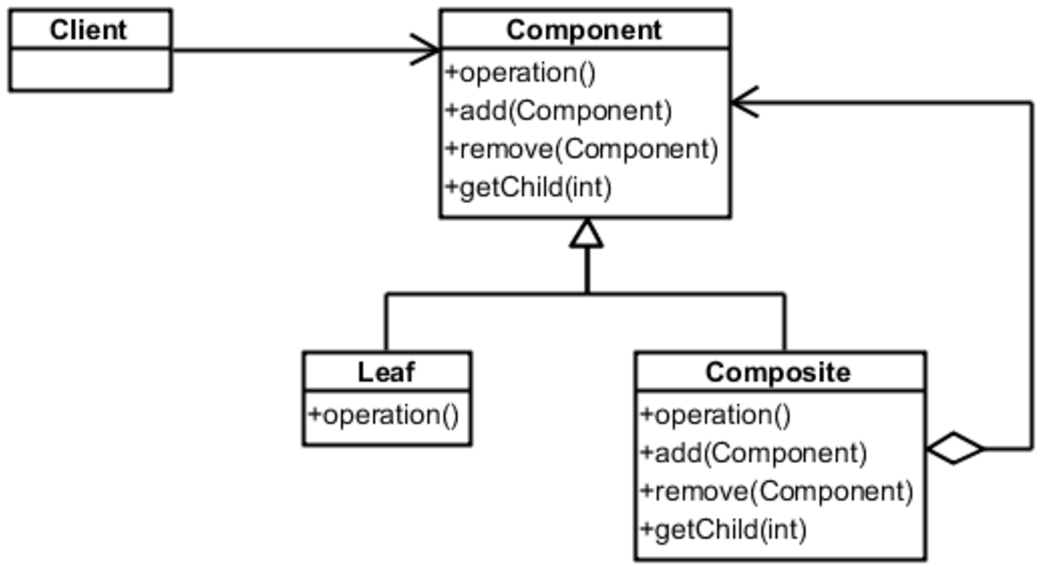
\includegraphics[width=0.6\textwidth]{composite.png}
    \attribution{Э. Гамма и др., Приемы объектно-ориентированного проектирования}
\end{center}

Клиент (то есть внешний по отношению к структуре объектов код) знает в основном только про общий базовый класс и пользуется его операциями при работе со всеми элементами дерева. <<В основном>> потому, что иногда клиенту (или какому-то из клиентов) всё-таки требуются специфические для какого-то конкретного класса операции и надо до них как-то добраться. В базовом классе же (обычно) определены и операции для манипуляции дочерними элементами, несмотря на то, что для листовых узлов они бессмысленны. Составные элементы содержат ссылки на элементы базового класса, чтобы внутри них могли лежать какие угодно элементы. Обратите внимание, что листовых и составных элементов может быть несколько разных классов, и они даже могут образовывать свои иерархии наследования (и часто делают это).

Итак,

\begin{itemize}
    \item паттерн описывает представление иерархии объектов вида часть-целое, крайне очевидным образом, но тут интересны детали, о которых чуть-чуть дальше;
    \item при этом паттерн в большинстве случаев позволяет обеспечить единообразость работы со всеми объектами в дереве, что существенно упрощает код;
    \item новые виды компонентов при таком подходе добавлять очень просто, это просто наследники либо общего предка (того, что на диаграмме Component), либо кого-то из более конкретных узлов --- клиентский код, скорее всего, даже не надо будет трогать.
\end{itemize}

На практике этот паттерн встречается очень часто --- оконные пользовательские интерфейсы, DOM\footnote{Document Object Model}-дерево в браузере, разобранные XML-документы в памяти, синтаксические деревья в компиляторах, и т.д. и т.п.

\subsection{Детали реализации}

Паттерн <<Компоновщик>> выглядит очевидной идеей, но на самом деле вообще плохо уживается с объектно-ориентированным программированием. Проблема в операциях по работе с дочерними элементами, типа вставки и удаления. Если их, как предлагалось выше, объявлять в Component, в Leaf для них невозможно предоставить адекватную реализацию, поскольку у Leaf нет дочерних элементов (получается известный code smell --- пустые переопределения методов). Если реализовать их только в Composite, то те клиенты, которым с дочерними элементами делать ничего не надо, будут счастливы, а остальным придётся делать преобразование типов.

Решить эту проблему красиво с точки зрения ООП не получится, можно лишь сделать достаточно хорошо:

\begin{itemize}
    \item если всё-таки методы определяются в Component, стоит в Leaf бросать исключения при попытке их вызвать --- чтобы программа сразу упала, если клиент пытается сделать то, что делать не должен, и мы могли бы быстро найти ошибку;
    \item иногда пустое поведение по умолчанию вполне удовлетворительно, тогда никаких исключений бросать не надо, а стоит просто смотреть на Leaf как на компонент, у которого есть дочерние элементы, просто их всегда 0. На таком подходе основан паттерн Null Object --- если мы не хотим всякий раз в коде, работающем с элементами дерева, проверять сыновей на null, мы просто заменяем отсутствующие узлы на фиктивные, но существующие узлы, которые просто ничего не делают.
    \item Если мы хотим всё-таки объявлять операции в Composite, то надо будет делать в клиентском коде проверку и преобразование типов, что неудобно. Чтобы клиенту было проще, можно в Component объявить операцию getComposite(), которая бы возвращала null для листьев и уже правильного типа Composite, если это Composite. Это в принципе то же, что преобразование типов, и проверку (на null) всё равно придётся делать в клиенте, но выглядит в коде это приятнее.
\end{itemize}

Похожая проблема --- это где определять список дочерних элементов. Обычно это делают в Composite, но можно делать и в базовом классе (Component), тогда всю машинерию по работе с потомками можно реализовать прямо в нём и не заставлять разные виды Composite этим заниматься. На практике часто бывает, что потомки имеют вполне определённую семантику, например, тип возвращаемого значения и параметры у узла <<Функция>> в синтаксическом дереве компилятора. Поэтому списки потомков определяются вообще в каждом конкретном потомке Composite, вместе с операциями, позволяющими с ними работать. Клиенту придётся знать точный тип узла, но в таком случае обычно это не проблема, потому что точный тип и так надо знать (см. паттерн <<Посетитель>> как пример общего решения этой проблемы). Кстати, обратите внимание, что список потомков вовсе не обязан быть списком --- это вполне может быть хеш-таблица, дерево или что угодно. Например, если у узла может быть сотня дочерних узлов разного предназначения, но в каждый конкретный момент времени непустых узлов мало, их вполне можно сложить в хеш-таблицу для экономии памяти, и обеспечить константную асимптотику доступа к нужному дочернему узлу. Так, например, работает подписка на события элементов управления в оконной библиотеке WPF\footnote{Windows Presentation Foundation}.

Несколько проще дела обстоят с хранением ссылки на родителя у дочерних узлов, хотя про это приходится думать каждому первокурснику, пишущему двоичные деревья. Ссылка на родителя может быть полезна для простоты обхода дерева и для реализации передачи ответственности от дочернего узла к родителю (см. паттерн <<Цепочка обязанностей>> --- так, опять-таки, часто устроена обработка событий в оконных библиотеках, если кнопка не может обработать событие клика, она передаёт его панели, на которой находится, та форме, и т.д.). Однако такая ссылка --- дополнительный инвариант, который надо поддерживать (что все дочерние элементы узла считают родителем этот узел), нарушение этого инварианта приводит к трудноотлавливаемым ошибкам при обходе и, опять же, ссылка память занимает. Тем более что обычно операции над деревом выполняются рекурсивно и можно родителя просто передавать в рекурсивный вызов как дополнительный параметр. Однако если ссылка на родителя всё-таки нужна, она нужна всем узлам, и поэтому её обычно делают прямо в Component.

Более интересный приём --- это использование разделяемых листьев или целых разделяемых поддеревьев. Например, тот же Null Object --- объект, который как бы есть, но ничего полезного не делает, может быть в памяти один. И если он в дереве встречается несколько раз, то все узлы, которые его используют, ссылаются на один и тот же объект. Да, это будет не совсем дерево уже, но поскольку объект всё равно ничего не делает, никто не заметит. Могут быть и более сложные случаи, например, компилятор может одинаковые подвыражения разделять между выражениями, в которых они встречаются, для экономии памяти (и улучшения скорости работы, ведь сборка мусора может изрядно её просадить). Если поддеревья и узлы немутабельны, разделять их может быть очень правильно. Однако и для мутабельных узлов можно кое-что придумать --- см. паттерн <<Приспособленец>>, там идея в том, что состояние делится на то, что можно безопасно разделять, которое хранится в узле, и на неразделяемое внешнее состояние, которое передают узлу при каждом вызове его операций. Разделяемые листья и поддеревья могут сильно сэкономить память, но делают невозможным использование ссылок на родителей и существенно усложняют работу с мутабельным состоянием.

Аналогичная оптимизация --- это кеширование информации для обхода или поиска в узлах. Например, в нашем текстовом редакторе мы могли бы для каждого глифа вычислять его ограничивающий прямоугольник и сохранять его в узле, и это позволило бы реализовать очень быструю операцию Intersects. Однако с кешированием есть общая проблема --- инвалидация кеша. Если в поддереве что-то поменялось, надо пересчитать кеши для всех родителей (или хотя бы пометить их как невалидные, чтобы при следующем запросе они пересчитались).

Ещё соображения, на которые может быть надо обратить внимание.

\begin{itemize}
    \item Порядок потомков может быть важен, а может быть нет --- например, порядок параметров в функции при передаче параметров по позиции критичен, а при передаче по имени не имеет значения. Это может радикально влиять на семантику дерева, так что это надо понимать, причём зачастую для каждого узла дерева отдельно --- для кого-то порядок фиксирован, для кого-то не важен.
    \item Управление памятью --- если нет сборки мусора, то за памятью в дереве надо аккуратно следить, особенно если используются разделяемые листья или поддеревья. Обычно Composite отвечает за удаление всего своего поддерева, а разделяемость реализуется очень аккуратным подсчётом ссылок. В языках со сборкой мусора всё проще, но если забыть занулить вовремя ссылку, в памяти может оказать гигантское никому не нужное дерево, которое сборщик мусора не может собрать. А в некоторых применениях паттерна <<Компоновщик>>, например, XML-базах данных, речь может идти о гигабайтах данных.
\end{itemize}

Итак, <<Компоновщик>> --- один из самых простых, известных и широкоиспользуемых паттернов, но (судя по количеству деталей реализации) оказывается, что аккуратное применение этого паттерна может быть не такой и простой задачей.

\section{Паттерн <<Декоратор>>}

\subsection{Мотивирующий пример}

Снова вернёмся к текстовому редактору. Теперь мы хотим сделать поддержку всяких украшательств пользовательского интерфейса, типа рамок вокруг области ввода текста, и полосы прокрутки. При этом хочется, чтобы пользователи могли включать-выключать по опции разные элементы пользовательского интерфейса, а в случае с полосой прокрутки --- иметь возможность и автоматически её добавлять/убирать в зависимости от количества текста. Причём так, чтобы другие части редактора даже не знали про то, есть там где-то полосы прокрутки или нет.

Вспомним (как мы решили в паттерне <<Компоновщик>>), что всё, что можно нарисовать на экране --- наследник класса Glyph, в том числе и страница с текстом. Первое решение, которое приходит в голову --- сделать ещё одного наследника Glyph, <<страница с текстом в рамке>>, а потом ещё одного, <<страница с текстом с полосой прокрутки>>. Но это не удобно, потому что вдруг мы захотим страницу и в рамке, и с полосой прокрутки. Да и поскольку наследование --- структура времени компиляции, менять во время выполнения обрамлённый текст на необрамлённый очень сложно. Поэтому наследование мы использовать не хотим, а хотим использовать композицию. 

Идея с наследованием от Glyph на самом деле всё-таки не так уж и плоха: мы можем сделать классы <<Рамка>> и <<Полоса прокрутки>> глифами, что позволит им вкладываться друг в друга и нисколько не противоречит архитектуре (всё, что можно нарисовать на экране --- наследник класса Glyph, а полосу прокрутки определённо можно нарисовать на экране). Это имеет тот побочный эффект, что рамки и полосы прокрутки могут появляться где угодно в тексте, а не только вокруг страницы --- но, возможно, это и не плохо, особенно в случае с рамками. Такой приём в книжке <<Банды Четырёх>> называется <<прозрачное обрамление>>, поскольку для всего внешнего мира глифы с рамками и без неразличимы, то же с полосами прокрутки.

Чтобы реализовать эту идею, добавим в нашу архитектуру класс MonoGlyph: абстрактный класс с ровно одним сыном, он будет базовым для всех видов <<обрамлений>>:

\begin{center}
    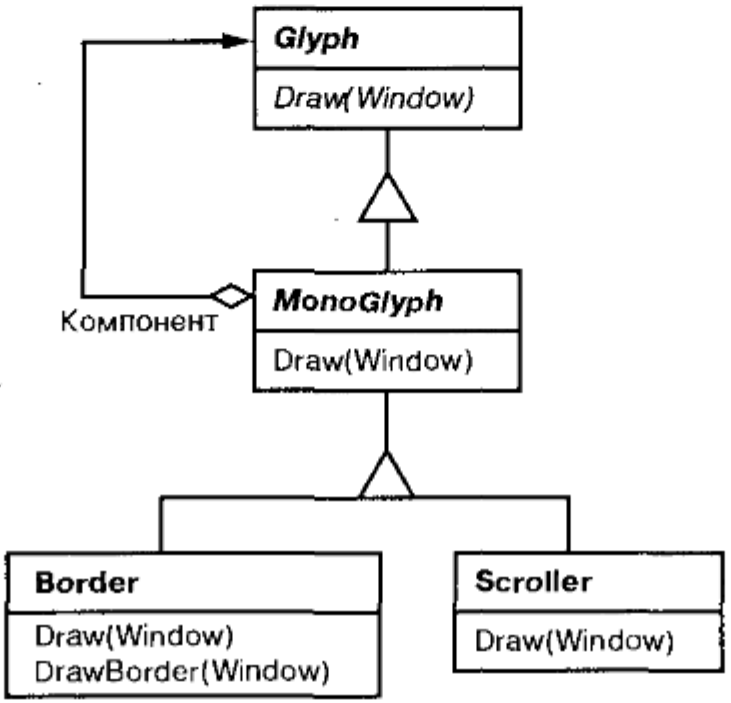
\includegraphics[width=0.4\textwidth]{monoglyph.png}
    \attribution{Э. Гамма и др., Приемы объектно-ориентированного проектирования}
\end{center}

Как можно заметить, это на самом деле вырожденный случай паттерна <<Компоновщик>> --- тут тоже объекты образуют иерархию включения, но моноглиф включает ровно один дочерний элемент, и цель этого --- не организация иерархии, а дополнение дочернего элемента новым поведением или состоянием. Во время выполнения структура объектов может выглядеть так:

\begin{center}
    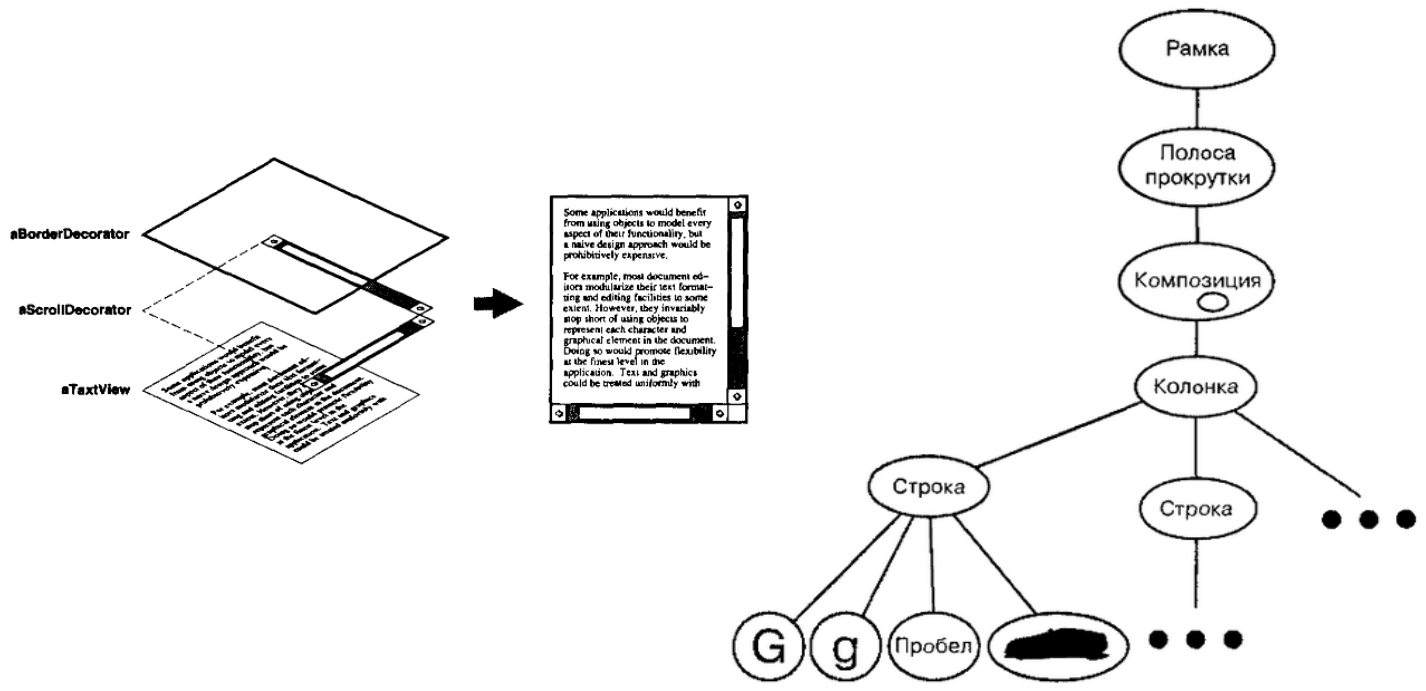
\includegraphics[width=0.9\textwidth]{glyphStructure.png}
    \attribution{Э. Гамма и др., Приемы объектно-ориентированного проектирования}
\end{center}

Эта структура позволяет вкладывать один элемент оформления в другой, что интересно ещё и тем, что в зависимости от того, в каком порядке что вкладывается, результат может быть разным. Если сначала рамка, а затем полоса прокрутки, то скроллится содержимое рамки. Если сначала Полоса прокрутки, затем рамка, то рамка сама скроллится, вместе с текстом.

\subsection{Декоратор (Decorator), общая структура}

Предложенную структуру классов можно обобщить до паттерна <<Декоратор>>:

\begin{center}
    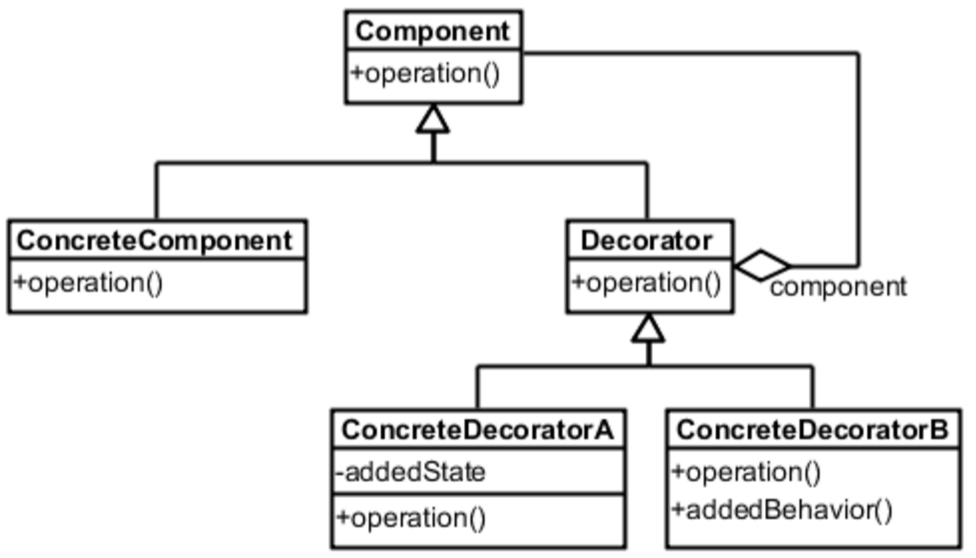
\includegraphics[width=0.55\textwidth]{decorator.png}
\end{center}

Декорировать можно как конкретные объекты (ConcreteComponent), так и другие декораторы, поэтому Decorator тоже наследуется от Component. Декоратор содержит в себе поле типа Component и вынужден (раз уж наследуется) определять все методы Component. Те, которые ему не интересны, он просто пересылает декорируемому объекту, а нужные методы (типа метода отрисовки в нашем примере с редактором) может переопределять. Или добавлять новые --- тогда те, кто ничего не знают про декоратор, могут пользоваться им прямо как декорируемым объектом и никогда не заметить разницы, а те, кто знает, могут сделать приведение типа и пользоваться новой функциональностью. Или новым состоянием, потому что и поля декоратор может иметь свои.

Это всё позволяет фактически менять поведение объекта во время выполнения, добавляя ему новые возможности или наоборот, удаляя их. Гораздо гибче, чем наследование, которое фиксируется во время компиляции и во время выполнения уже ничего не изменить. Возможность добавлять новое состояние и поведение позволяет не пытаться определить всё в базовом классе, а вынести часть функциональности в декораторы, про которые будут знать только те, кому эта функциональность нужна (и делать преобразования типов, что не очень объектно-ориентировано, но неплохо работает на практике). Однако за гибкость приходится платить --- во время выполнения оказывается много мелких объектов вместо одного большого, что приводит к дополнительным накладным расходам по памяти (да и по времени, лишние полиморфные вызовы не выполняются даром).

\subsection{Детали реализации}

Декоратор имеет довольно близкий паттерн <<Адаптер>>, который также оборачивает один объект в другой объект, но в <<Адаптере>> интерфейсы этих объектов не совпадают (поэтому он и <<Адаптер>> --- адаптирует один интерфейс для клиентов, которые хотят другой). Идея декоратора именно в том, чтобы реализовывать интерфейс декорируемых объектов, чтобы внешний мир думал, что декоратора вообще нет, и со структурой данных можно работать как обычно.

Это влечёт тот факт, что класс Component должен быть небольшим, во-первых, по количеству объявленных в нём методов: потому что мы замучаемся их переопределять, даже если переопределение для большинства из них --- это просто вызов метода декорируемого объекта, в одну строчку. Во-вторых, он должен быть небольшим по объёму хранимых в нём данных, потому что декоратор, наследуясь от Component, получает не только все его методы, но и все его поля --- и не использует их никак, ведь он просто перенаправляет запросы декорируемому объекту. Кстати, начинающие программисты часто путаются: меняют поле декоратору, а ничего не происходит --- потому что на самом деле с полем работает декорируемый объект, спрятанный в декораторе, а у него \textit{свой} набор полей. Поэтому в идеале Component должен быть вообще интерфейсом и никакого состояния не иметь.

Если это не так и Component --- это полноценный большой класс с кучей методов, лучше подойдёт паттерн <<Стратегия>>. Это как декоратор наоборот, он не надевается поверх объекта, а вкладывается в объект. Когда объекту надо выполнить какое-то действие, он обращается к стратегии и она делает за него работу. Но стратегия, в отличие от декоратора, требует, чтобы мы заранее знали, какие действия мы позволяем параметризовать с помощью стратегии, а какие нет, поэтому декоратор гибче. 

Ещё распространённый приём, более легковесный, чем <<Стратегия>> --- это заранее определить в Component набор точек расширения (<<hooks>> в англоязычной литературе), и вызывать их перед/после/во время выполнения действия. По умолчанию <<хуки>> просто ничего не делают, но если их переопределить (отнаследовавшись от Component или передав <<хуки>> как лямбда-функции), они могут модифицировать действие, как им захочется, вплоть до полной его отмены. Опять-таки, при написании Component надо заранее подумать о точках расширения, тогда как декоратор не требует в Component никаких изменений вовсе\footnote{Это не совсем правда: в C\# или C++ методы по умолчанию не виртуальные, так что если в Component не написано явно, что их можно переопределять, декоратор написать не получится. В Java методы по умолчанию виртуальные, так что там шансов больше, но Component может испортить авторам декоратора жизнь, используя final.}, поэтому гораздо гибче.

\section{Паттерн <<Стратегия>>}

\subsection{Мотивирующий пример}

Следующая задача в нашем текстовом редакторе --- алгоритмы форматирования текста. Хочется иметь механизм, размещающий текст на странице с учётом пожеланий пользователя, таких как количество колонок, ширина полей, размер абзацного отступа и т.д. При этом, поскольку у нас WYSIWYG-редактор, мы хотим, с одной стороны, чтобы оно работало в реальном времени, с другой стороны --- чтобы результат получался посимпатичнее. 

Продвинутые редакторы, типа TeX, учитывают даже такие параметры, как <<цвет>> документа (то есть соотношение пробелов и непробельных символов) и следят за тем, чтобы пробелы в соседних строках не выстраивались в одну колонку (чтобы текст визуально не разделялся надвое). WYSIWYG-редакторы обычно не могут себе такого позволить, поскольку форматирование вызывается после каждой напечатанной буквы, но кажется хорошей идеей дать возможность самому пользователю выбрать, получше сделать или побыстрее. Например, пока пользователь просто набирает текст, используется быстрый алгоритм форматирования, а когда уже верстает начисто, медленный, но дающий красивый результат.

Поэтому мы приходим к идее вынести алгоритм форматирования в отдельный класс, сделать для него интерфейс, и реализовать этот интерфейс несколькими разными алгоритмами. Чтобы встроить всё в систему, как обычно, отнаследуемся от класса Glyph, добавив <<псевоглиф>> Composition:

\begin{center}
    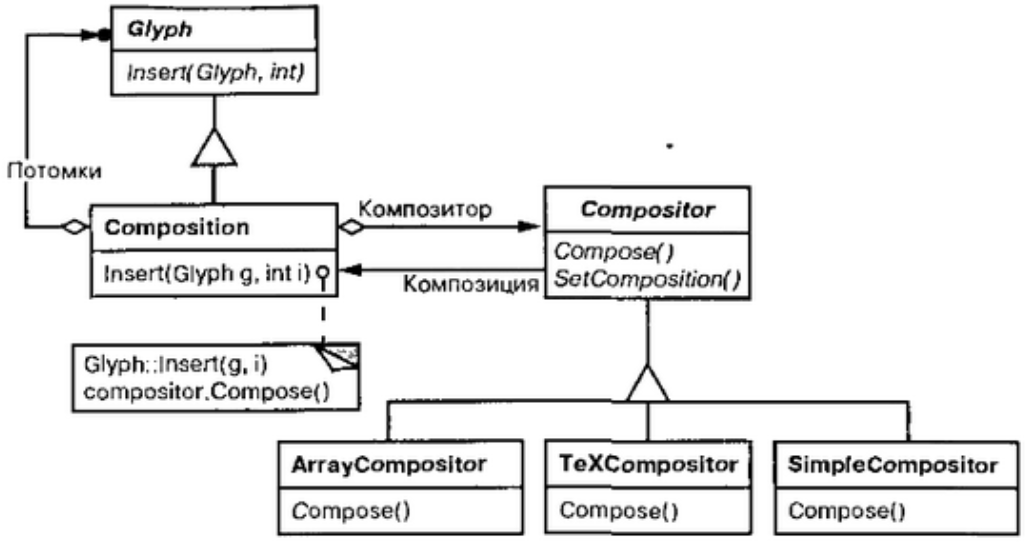
\includegraphics[width=0.7\textwidth]{compositor.png}
    \attribution{Э. Гамма и др., Приемы объектно-ориентированного проектирования}
\end{center}

Теперь, когда кто-то вызывает Insert у строки, на которую навешен Composition, она дёргает выбранный алгоритм композиции (точнее, его метод Compose), который добавляет межсимвольные интервалы, а если Insert вызван у страницы, обёрнутой в Composition, вызывается разбивка на колонки и т.д. Алгоритму нужны данные, с которыми он бы работал, поэтому у него ещё есть метод SetComposition, куда можно передать то, что ему, собственно, надо композировать.

\subsection{Стратегия (Strategy), общая структура}

Это всё обобщается до паттерна <<Стратегия>>, основное назначение которого --- инкапсуляция алгоритма в объект, так, чтобы алгоритм можно было легко прямо во время выполнения заменить, и чтобы его сложность не мешала всей остальной системе:

\begin{center}
    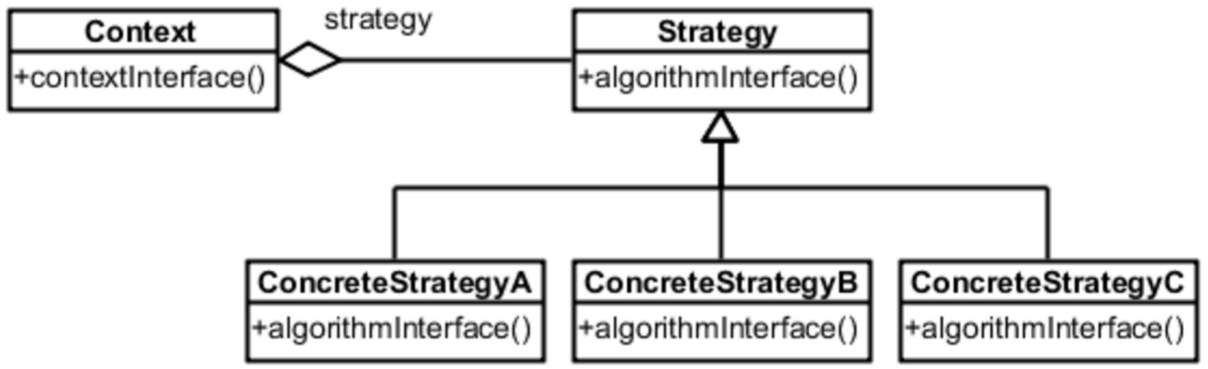
\includegraphics[width=0.7\textwidth]{strategy.png}
\end{center}

Context содержит стратегию как поле по интерфейсу Strategy. Когда пользователям что-то надо от Context, он делегирует запрос Strategy, и его исполняет объект конкретной стратегии, который сейчас у Context. Если стратегию надо поменять, то Context просто передают новый объект-стратегию, и он начинает перенаправлять запросы ему.

Хорошо это, если:

\begin{itemize}
    \item как в нашем примере с форматированием текста, имеется несколько разных алгоритмов, между которыми надо уметь легко переключаться;
    \item когда есть близкие по смыслу классы с разным поведением --- возможно, их можно зарефакторить так, чтобы само поведение вынести в стратегии, а сами классы склеить в один (Context в паттерне);
    \item когда класс всего один, но алгоритм сложный, состоит из нескольких этапов (которые можно вынести в private-методы), содержит вспомогательные данные (например, кеш), о которых не хочет знать контекст;
    \item в коде много условных операторов --- возможно, его можно зарефакторить, заменив условные операторы полиморфными вызовами стратегии.
\end{itemize}

\subsection{Детали реализации}

Первый и самый творческий момент при использовании паттерна <<Стратегия>> --- это проектирование его интерфейса (и интерфейса Context). Это надо сделать так, чтобы, с одной стороны, стратегии было остаточно информации для работы, с другой стороны, чтобы интерфейс не приходилось переделывать под каждую новую стратегию. В этом плане наиболее важно решить, как в стратегию передаётся необходимая для работы информация:

\begin{itemize}
    \item как параметры метода стратегии --- тогда стратегия может вообще ничего не знать про Context, но ей, скорее всего, придётся получать много лишних данных --- ведь не всем реализациям стратегии все аргументы потребуются;
    \item передавать сам Context в качестве аргумента, в надежде, что каждая стратегия сможет при необходимости спросить у него нужные ей данные --- это делает реализации стратегий более гибкими, но добавляет круговую зависимость между стратегией и контекстом, кроме того, заставляет контекст предоставлять интерфейс для доступа к данным, что плохо с точки зрения инкапсуляции.
\end{itemize}

Выбор, как обычно, зависит от конкретной ситуации и его должен сделать архитектор. Можно передавать аргументы и не в метод при вызове, а в конструктор стратегии, но обычно стратегия не имеет собственного состояния (кроме, быть может, кешей), так что это может быть плохой идеей. Почему --- стратегия может быть разделяемой: один объект-стратегия может обслуживать сразу много контекстов. Может быть разумно сделать стратегию приспособленцем из паттерна <<Приспособленец>> (о котором дальше) --- часть состояния, общую для всех обслуживаемых контекстов, стратегия хранит сама, часть передаётся извне при каждом вызове. И при этом есть единое место в системе, где каждый контекст может взять себе стратегию, когда ему надо.

Стратегия, кстати, может быть параметром шаблона, что особенно полезно в C++, поскольку там шаблоны раскрываются во время компиляции и это позволяет избежать оверхеда на виртуальные вызовы и хранение полей, неизбежного при использовании интерфейса Strategy. Так очень часто делает стандартная библиотека C++ --- например, аллокаторы часто передаются как параметры шаблона классам, которым они нужны. Естественно, такой приём можно использовать только тогда, когда стратегию не надо менять во время выполнения.

Ещё один немаловажный аспект применения этого паттерна --- при наивной реализации контекст будет падать, если стратегию случайно забыли выставить. С этим можно бороться, выставляя стратегию по умолчанию в конструкторе Context, либо просто if (стратегия установлена) вызвать-стратегию() else делать-что-то. Стратегия или поведение по умолчанию может обеспечивать базовую функциональность Context, а если пользователя это не устраивает, он может подсунуть ему свою стратегию.

И последнее замечание --- лямбда-функция тоже объект, и тоже созданный, чтобы инкапсулировать действие. Поэтому в современных языках лямбда-функции хорошо подходят для реализации простых стратегий, у которых всего один метод в интерфейсе. Благодаря замыканиям (closure), лямбда-функции даже могут иметь своё состояние и общаться с внешним миром.

\section{Паттерн <<Адаптер>>}

\subsection{Мотивирующий пример}

Следующий паттерн разберём на другом, но близком, примере --- допустим, мы хотим написать графический редактор. Допустим, более того, что большую часть мы уже написали --- у нас есть GUI, поддержка графических примитивов типа линий, прямоугольников и т.д., и нам надо добавить поддержку текста на изображении. Можно, конечно, реализовать её самим, но это в разы сложнее, чем весь редактор вместе взятый --- поддержка разных шрифтов, размеров, начертаний и т.д. и т.п. Поэтому предположим, что мы, как все нормальные архитекторы, нашли стороннюю библиотеку, которая умеет рисовать текст на канве, и хотим её использовать в нашем редакторе. Но, поскольку библиотека сторонняя, она про наш редактор ничего не знает, так что лихо добавить текстовое поле как ещё одну фигуру в наш редактор не получится. Нам нужна некая прослойка, которая бы оборачивала сторонний класс в нашу инфраструктуру --- это и есть паттерн <<Адаптер>>:

\begin{center}
    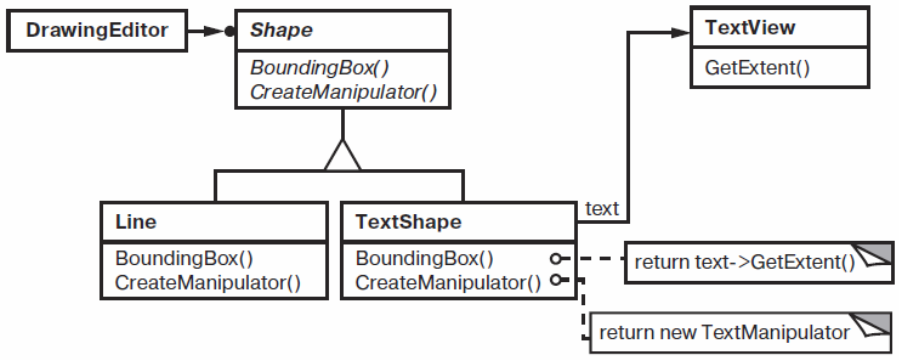
\includegraphics[width=0.7\textwidth]{adapterExample.png}
    \attribution{Э. Гамма и др., Приемы объектно-ориентированного проектирования}
\end{center}

DrawingEditor тут --- некий GUI нашего редактора, Shape --- интерфейс для всего, что можно нарисовать на канве, включая всякие примитивы и TextShape --- тот самый адаптер. TextShape сам ничего не делает, его единственная работа --- это реализовывать интерфейс Shape и делегировать все запросы библиотечному классу TextView, который как раз нам и нужен. TextShape, если потребуется, может иметь и какую-нибудь нетривиальную логику преобразований или даже новую функциональность относительно адаптируемого объекта --- например, наш редактор хочет у каждой фигуры элемент управления, за который её можно подвигать/повращать, и его возвращает CreateManipulator. Тем не менее, в основном содержательная логика находится в адаптируемом объекте, в нашем случае в TextView.

\subsection{Адаптер (Adapter), общая структура}

Эта идея обобщается в следующую структуру:

\begin{center}
    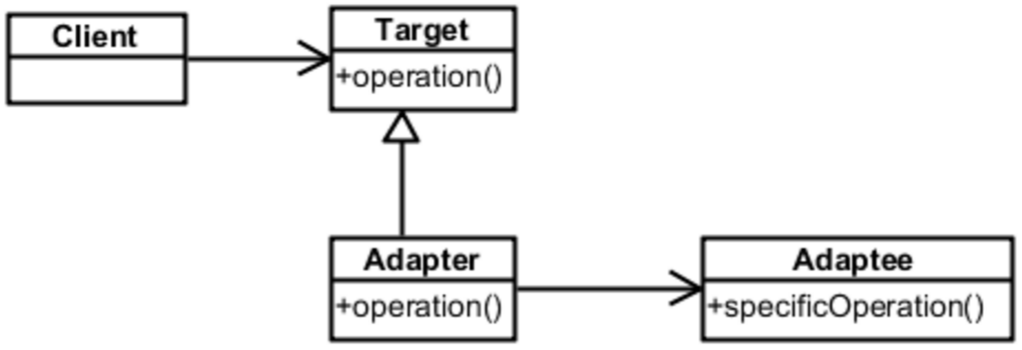
\includegraphics[width=0.55\textwidth]{objectAdapter.png}
\end{center}

Тут Client ожидает некий интерфейс Target, которому не удовлетворяет класс Adaptee, поэтому мы делаем класс Adapter, который реализует интерфейс Target и использует для его реализации Adaptee, просто перенаправляя ему запросы и, быть может, правильно преобразуя их (возможно, нетривиально --- одно действие Target вполне может реализовываться несколькими методами Adaptee).

Эта реализация называется <<Адаптер объекта>> в противоположность другому способу сделать то же самое --- <<Адаптеру класса>>:

\begin{center}
    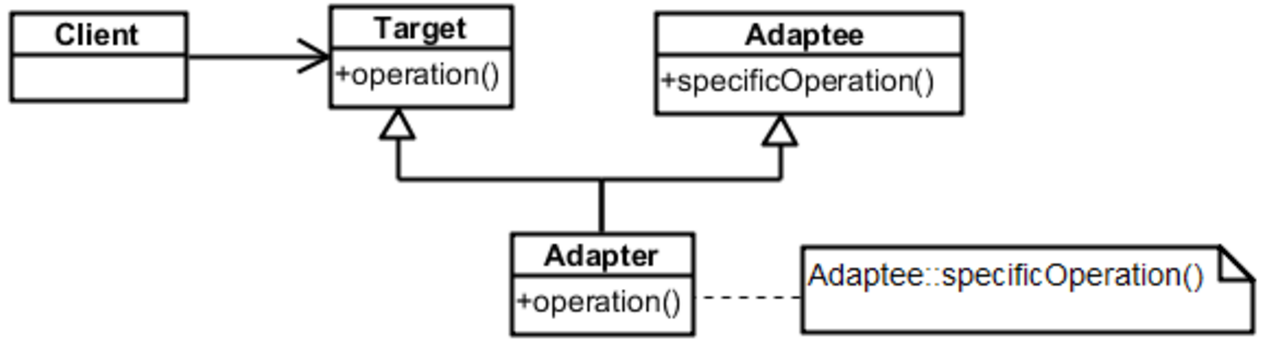
\includegraphics[width=0.65\textwidth]{classAdapter.png}
\end{center}

Здесь Adapter наследуется от Adaptee и реализует интерфейс Target, вызывая методы своего предка. Обычно это пишется несколько короче, чем адаптер объекта, поскольку не требуется указывать имени поля при вызове метода (методы Adaptee --- это на самом деле и методы Adapter, так что их можно вызывать напрямую). Но не очень гибко, а если Target не интерфейс, а абстрактный класс, и вовсе требует множественного наследования.

\subsection{Детали реализации}

Паттерн весьма прямолинейный, поэтому единственная тонкость реализации, достойная упоминания --- это то, что для реализации адаптера класса может быть эффективно использовано private-наследование C++ (и это, пожалуй, единственный известный пример, когда private-наследование кому-нибудь нужно). Adapter не должен реализовывать интерфейс Adaptee (хотя бывают двусторонние адаптеры, но это редкость), он только использует его методы, поэтому он может скрыть эти методы от внешнего мира механизмом private-наследования. При private-наследовании все поля и методы предка становятся private-полями и методами потомка, вне зависимости от их модификаторов доступа у предка. Естественно, это противоречит принципу подстановки Лисков, поскольку потомок контракт предка не выполняет, поэтому в современных языках такого нет. Но в C++ есть, и вот тут это может немножко улучшить инкапсуляцию. Но поскольку адаптер объекта в большинстве случаев всё равно предпочтительнее, это не так важно.

\section{Паттерн <<Заместитель>>}

\subsection{Мотивирующий пример}

Вернёмся к текстовому редактору. У нас, как и у любого нормального редактора, должна быть функциональность добавления в документ изображений. Однако изображения могут быть большими, и документы могут быть большими, так что загрузка всех изображений с диска при открытии документа может быть довольно заметна по времени\footnote{Широкое распространение SSD-дисков делает этот пример не таким актуальным, как задумывала Банда Четырёх, но представьте себе, что речь идёт о браузере и подгрузке изображений со сторонних ресурсов}. Поэтому мы можем поступить хитрее --- грузить картинку только в тот момент, когда пользователь долистает до страницы, на которой картинка находится. Если документ большой, то с большой вероятностью большинство изображений не придётся грузить вообще никогда.

Но есть одна проблема --- чтобы правильно разбить документ на страницы, алгоритму форматирования надо знать размеры изображений. Поэтому при открытии документа нам надо всё-таки пробежаться по изображениям, узнать их размер (например, быстро считав заголовки файлов) и создать на месте изображений в тексте глифы-<<заглушки>>, которые бы знали размер настоящего изображения и умели его при необходимости грузить. Тогда алгоритм форматирования сможет правильно сверстать весь текст (так что пользователь будет точно знать, сколько страниц в документе), а полное чтение изображения будет выполняться только когда пользователь открыл страницу:

\begin{center}
    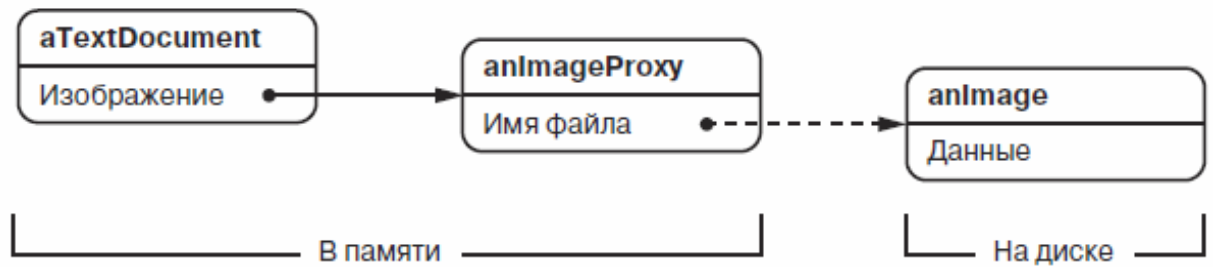
\includegraphics[width=0.75\textwidth]{proxyExample.png}
    \attribution{Э. Гамма и др., Приемы объектно-ориентированного проектирования}
\end{center}

Структурно это всё устроено вот так:

\begin{center}
    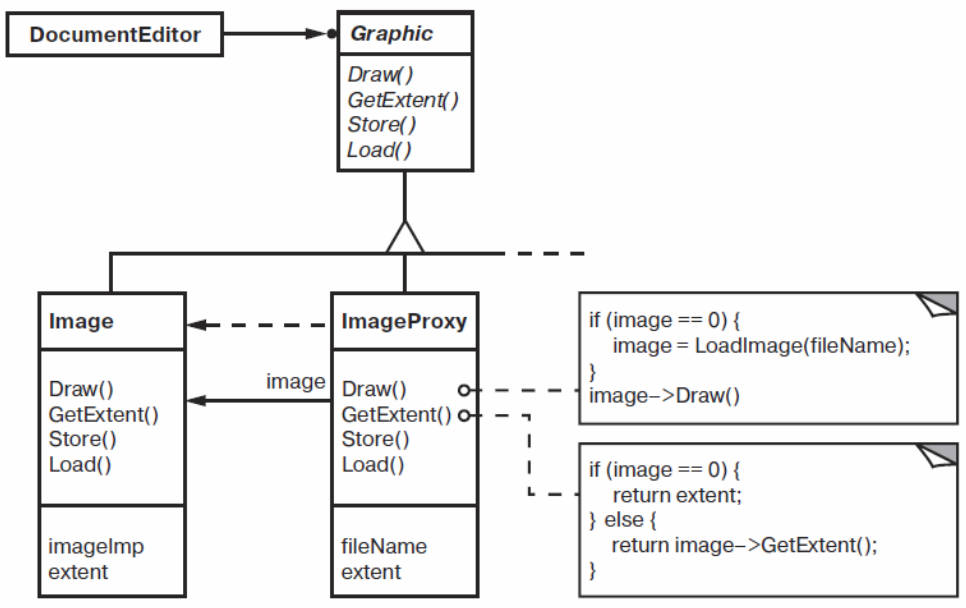
\includegraphics[width=0.75\textwidth]{proxyExampleClassDiagram.png}
    \attribution{Э. Гамма и др., Приемы объектно-ориентированного проектирования}
\end{center}

Положим, Graphic --- это наследник Glyph из предыдущих примеров, который отвечает за работу с изображениями. Его, помимо всяких других вещей типа диаграмм, графиков и автофигур, реализует класс Image, и тот самый объект-<<заглушка>> --- ImageProxy. ImageProxy хранит в себе ссылку на Image, изначально она null, имя файла, откуда при необходимости надо изображение загрузить, и его размер, прочитанный заранее из этого файла. Поскольку ImageProxy реализует тот же интерфейс, что и Image, для всего внешнего мира ImageProxy от Image неотличим. Когда внешний мир вызывает методы, которые ImageProxy может реализовать сам (типа получения размера), он реализует их сам, когда дело доходит до содержательной работы, ImageProxy создаёт и загружает Image из файла и начинает перенаправлять все запросы к нему.

\subsection{Заместитель (Proxy), общая структура}

То, что мы реализовали выше, на самом деле называется <<Замещающий прокси>>. В общем случае паттерн устроен вот так:

\begin{center}
    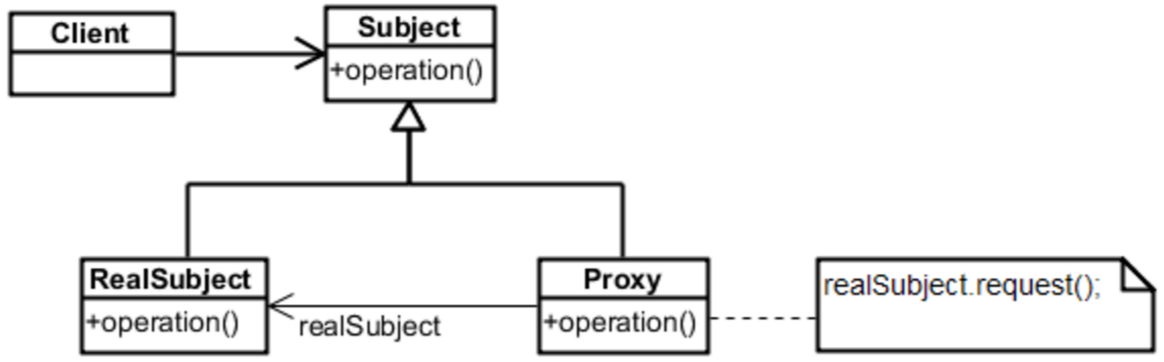
\includegraphics[width=0.68\textwidth]{proxy.png}
\end{center}

Proxy всегда реализует тот же интерфейс, что и проксируемый объект (как паттерн <<Декоратор>>), и имеет способ добраться до реального объекта или создать его при необходимости (и тем отличается от декоратора --- прокси обычно ссылается на конкретный класс, так что надеть прокси на прокси не получится, но и не надо). Proxy подменяет реальный объект и сам выполняет те запросы, что может, а что не может --- перенаправляет реальному объекту.

Используется этот паттерн очень много где, вот частные случаи его применения:

\begin{itemize}
    \item представление объектов, физически находящихся на другом компьютере;
    \item отложенная загрузка, ленивое создание <<тяжёлых>> объектов;
    \item контроль доступа к объекту;
    \item возможность подменить объект на другой, не исправляя ссылки в тысяче других объектов, которые хотят им пользоваться;
    \item умные указатели и разные вариации на их тему:
    \begin{itemize}
        \item подсчёт ссылок,
        \item ленивая загрузка/инициализация,
        \item работа с блокировками в многопоточных программах,
        \item копирование при записи (copy-on-write, известный приём экономии вычислительных ресурсов).
    \end{itemize}
\end{itemize}

Как видим, паттерн <<Заместитель>> (его столь же часто <<переводят>> просто как <<Прокси>>) используется везде. \textit{Практически любое} распределённое приложение использует клиенты для работы с удалёнными сервисами --- ни что иное, как прокси. \textit{Практически любая} программа на C++ использует умные указатели --- прокси. В стандартной библиотеке любого нормального языка есть механизм отложенных вычислений (Lazy) или вычислений, которые завершатся когда-либо в будущем (Future/Promise/Task, везде по-разному) --- прокси.

\subsection{Детали реализации}

Тонкости реализации этого паттерна сильно зависят от сферы его применения, но общая для всех проблема --- это тот факт, что прокси должен полностью реализовать интерфейс проксируемого объекта, а он может быть весьма громоздким (у паттерна <<Декоратор>>, впрочем, тоже есть такая проблема). 

Например, для умных указателей это обходится одной странной особенностью языка C++ (есть подозрение, что сделанной в языке специально для этого): оператор разыменования и доступа к члену класса (\mintinline{c++}|->|) можно перегружать, и если этот оператор возвращает объект, у которого тоже есть оператор \mintinline{c++}|->|, тут же вызывается он, и так далее до тех пор, пока \mintinline{c++}|->| не вернёт объект, у которого \mintinline{c++}|->| нет. Например, \mintinline{c++}|object->do()| вполне может оказаться \mintinline{c++}|((object.operator->()).operator->()).do()|. То есть первый оператор \mintinline{c++}|->| вернул нам объект, у которого есть оператор \mintinline{c++}|->| (сырой указатель), он вызвался и вернул нам разыменованный объект, у которого уже нет оператора \mintinline{c++}|->|, и у него уже вызвался метод \mintinline{c++}|do()|. Собственно, умные указатели --- это обычные C++-ные классы, которые как раз и перегружают \mintinline{c++}|->|, чтобы та возвращала <<неумный>> указатель --- проксируемый объект. Так что для всего внешнего мира использование сырого и умного указателя при вызове метода никак не отличается и приводит к одинаковым результатам. Никто не мешает вам использовать тот же приём при реализации своих прокси, но если вам надо различать вызываемые методы (например, для организации контроля доступа или чего-то ещё), такой способ вам никак не поможет --- оператор \mintinline{c++}|->| всего один, и он не знает, что написано справа от него.

Если методы всё-таки надо различать или они не просто перенаправляют запрос проксируемому объекту, их часто всё-таки приходится писать вручную (поэтому, так же, как и в случае <<Декоратора>>, удобно, когда интерфейс проксируемого объекта небольшой). Это выглядит довольно ужасно, особенно если большинство методов просто перенаправляют запрос --- получаются классы в сотню методов, каждый по одной строчке, которые очень скучно писать. Немного помогает то, что в современных языках делегирование запроса можно записать компактно, например, в C\#/F\#: \mintinline{csharp}|public void do() => realSubject.do();|. 

Однако работа по написанию таких прокси не требует интеллекта, а поэтому автоматизируема. Особенно если речь идёт про удалённые прокси (представляющие объект, размещённый на другой машине), часто применяется кодогенерация. Хороший пример --- это технологии наподобие Windows Communication Foundation или Swagger Codegen, где по описанию веб-сервиса, автоматически получаемого с самого веб-сервиса, генерируется прямо целый прокси-клиент, который собирается вместе с кодом клиентского приложения и используется там как обычный класс, будто он находится на машине клиента. В случае с WCF это особенно эффектно --- при наличии запущенного веб-сервиса со включённой публикацией метаинформации создание рабочего клиента --- дело пары минут и нескольких кликов мышью в Visual Studio.

Ещё одна тонкость, которую надо иметь в виду при реализации прокси, особенно при реализации отложенной загрузки, ленивых вычислений и т.д. --- что проксируемого объекта может и не быть в памяти. В этом случае наивная реализация в духе \mintinline{csharp}|public void do() => realSubject.do();| приведёт к куче Null Reference Exception. Как с этим бороться, мы видели на примере прокси для изображений в текстовом редакторе --- просто проверять каждый раз, есть ли у нас объект. Но вот надо про это помнить.

\section{Паттерн <<Фасад>>}

\subsection{Мотивирующий пример}

Положим, у нас есть компилятор какого-то языка, и мы хотим его использовать в своей программе\footnote{Например, многие компьютерные игры позволяют писать скрипты как часть игрового процесса, некоторые даже предлагают пользователю попрограммировать на C\# прямо внутри игры}, а ещё лучше, сделать его переиспользуемым, чтобы кто угодно мог встраивать его в свой код и использовать для своих целей (например, компилятор C\# с открытым исходным кодом, Roslyn\footnote{Roslyn на GitHub, URL: \url{https://github.com/dotnet/roslyn} (дата обращения: 20.08.2021г)}). Однако парсеры обычно довольно сложны: есть лексический анализатор, синтаксический анализатор, узлы абстрактного синтаксического дерева, анализатор типов и другие семантические анализаторы, разные оптимизаторы и генераторы кода для разных целевых платформ. Причём, каждая из этих частей может быть гибко конфигурируема (например, лексер может работать с файлами в разных кодировках). Переиспользование такой системы сильно страдает от того, что нам надо каждый раз создавать кучу классов, передавать им непонятные параметры и заставлять потом работать вместе, в правильном порядке вызывая их методы. А если нам надо просто скомпилировать и запустить программу и мы не хотим только ради этого слушать целый курс по языкам и трансляциям?

Идея решения довольно очевидна: а давайте сделаем класс, который будет сам собирать и запускать синтаксический анализатор, используя параметры по умолчанию. У этого класса есть только один метод Compile(), который и делает всю работу, полностью пряча сложность подсистемы компиляции от пользователя:

\begin{center}
    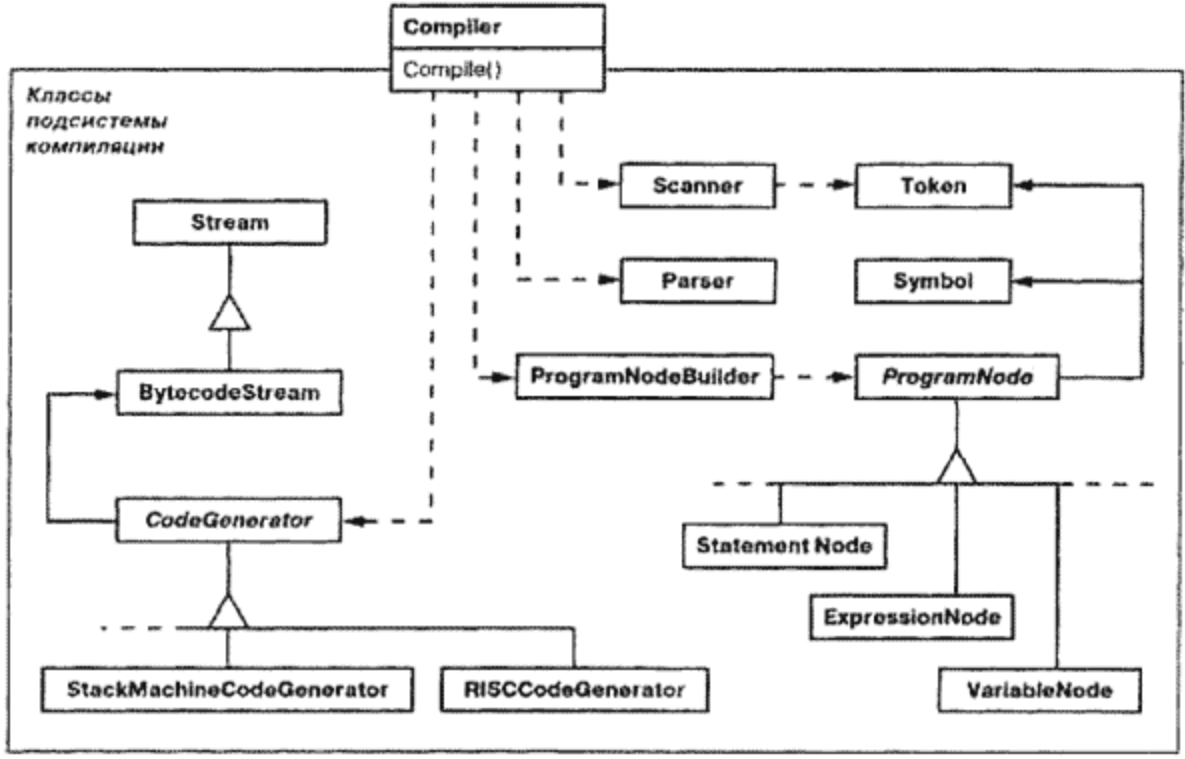
\includegraphics[width=0.8\textwidth]{facadeMotivation.png}
    \attribution{Э. Гамма и др., Приемы объектно-ориентированного проектирования}
\end{center}

При этом все внутренности подсистемы компиляции пользователю всё ещё доступны, и если поведение по умолчанию его не устраивает, он вполне может влезть внутрь или вообще не пользоваться фасадом.

\subsection{Фасад (Facade), общая структура}

Это соображение обобщается до паттерна <<Фасад>> с очень простой структурой:

\begin{center}
    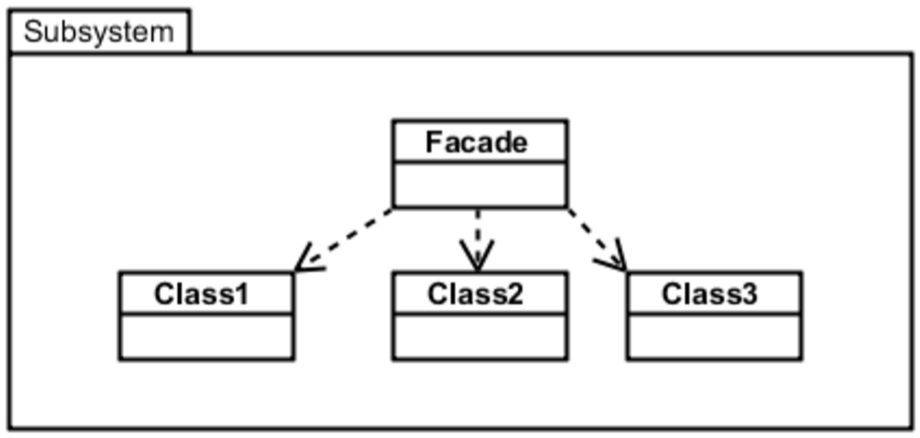
\includegraphics[width=0.5\textwidth]{facade.png}
\end{center}

Для потенциально большой и сложной подсистемы создаётся класс, единственная задача которого --- облегчить пользование этой подсистемой и предоставить внешнему миру простой и красивый интерфейс к ней. Применяется как в чисто утилитарных целях упрощения переиспользования, так и в более архитектурных --- отделения подсистем друг от друга. Фасад может и запрещать доступ к внутренним классам подсистемы, так что архитектурно представляет собой чёткую границу подсистемы, и контракт, который эта подсистема обязуется выполнять. Например, для многоуровневых архитектур --- каждый уровень может быть довольно сложен, но иметь фасад, и все уровни выше взаимодействуют с уровнем только через фасад, что позволяет добиться хорошей инкапсуляции и разделения ответственности. Однако этот паттерн не всегда применим --- если в фасаде получатся десятки несвязных методов, то использовать его не стоит.

\subsection{Детали реализации}

Паттерн очень простой, поэтому детали реализации долго обсуждать не получится. Полезный приём --- делать фасад абстрактным классом или интерфейсом (<<Абстрактный фасад>>), и предоставлять фабрику (паттерн <<Абстрактная фабрика>> или <<Фабричный метод>>) для того, чтобы порождать конкретный фасад. Это позволяет клиенту подсистемы не знать вообще ни про один конкретный класс, кроме очень простой фабрики, что способствует снижению связности. Плюс можно очень легко заменить подсистему, реализовав другой фасад с тем же интерфейсом. Стоит ли городить такой огород в каждом конкретном случае --- как обычно, решать вам.

Ещё паттерн <<Фасад>> не запрещает доступ к классам внутри подсистемы (и в книжке излагается именно такой вариант), но на практике часто полезно всё-таки делать фасад единственной точкой доступа к подсистеме. Это внезапно нетривиально даже в современных языках и часто сводится к непроверяемым компилятором соглашениям между программистами. Например, фасад может быть единственным public-классом пакета, а все остальные классы можно объявить как внутренние (большинство компилируемых языков имеют механизм разграничения видимости по пакетам/сборкам, но не все --- например, в C++ ничего такого нет). Однако если подсистема достаточно сложна и её тоже хочется разделить на пакеты, этот способ не помогает, потому что либо класс public для всех, включая пользовательский код, либо внутренний для всех, и не видим из других пакетов подсистемы. В таком случае применяют соглашения об именовании пакетов или пространств имён --- например, в C++ пространство имён details обычно используется для классов реализации подсистемы и клиентский код должен честно-честно не пользоваться классами оттуда. В стандартной библиотеке Java тем же целям служат пакеты с именем internal. Однако компилятор это не проверяет, поэтому для Java нередки ситуации, когда программа перестаёт компилироваться с выходом новой версии языка (естественно, виноваты при этом разработчики, и некоторые IDE, которые иногда автоматически импортируют первый попавшийся пакет с искомым классом, а разработчики слишком им доверяют, чтобы поправить).

\section{Паттерн <<Приспособленец>>}

\subsection{Мотивирующий пример}

Вернёмся к нашему текстовому редактору. Вспомним, что всё, что можно нарисовать на экране --- это глиф, в том числе каждая буква. Чтобы нарисовать букву, надо знать её шрифт, размер, начертание, цвет и т.п. При этом мы, конечно, хотим работать с каждой буквой как с отдельным объектом, это удобно, единообразно, и когда мы проектировали внутреннюю структуру документа в паттерне <<Компоновщик>>, решили делать именно так. Однако документы бывают большими (состоящими из миллионов букв), а миллионы мелких объектов сильно расстроят подсистему управления памятью (особенно в языках со сборкой мусора), что приведёт к чудовищному снижению производительности, да и тратить пару гигабайт оперативной памяти на открытие документа никто не захочет. Получается конфликт между красивой объектно-ориентированной архитектурой и реальностью, который обычно разрешается в пользу реальности, но тут можно придумать и ещё кое-что.

Идея такая: давайте не будем хранить честно каждую букву в тексте как отдельный объект, а сделаем пул букв (по одной на каждую букву алфавита, плюс прописные-строчные) и будем ссылаться из документа на буквы из пула, то есть если в строке 10 раз встречается буква <<а>>, то это будет просто 10 ссылок на один и тот же объект:

\begin{center}
    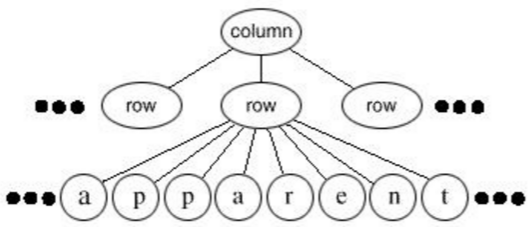
\includegraphics[width=0.38\textwidth]{noFlyweight.png}
    \raisebox{0.1\textheight}{\quad\Huge{$\rightarrow$}\quad}
    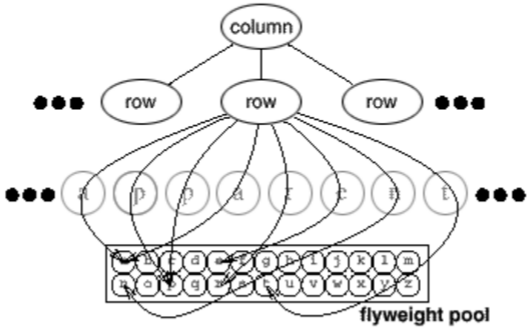
\includegraphics[width=0.38\textwidth]{flyweightExample.png}
    \attribution{Э. Гамма и др., Приемы объектно-ориентированного проектирования}
\end{center}

Однако, как мы писали ранее, у букв есть ещё шрифт, начертание, цвет и т.д., а при такой схеме получится, что все буквы <<а>> в тексте будут выглядеть совершенно одинаково. Не проблема, давайте хранить атрибуты букв, которые в разных местах могут быть разные, в самих этих местах (например, в строке), а когда букву надо отрисовать или ещё что-то с ней сделать, передавать ей всё необходимое. Это как раз то, почему паттерн называется <<Приспособленец>>, а не просто разделяемый объект --- объекты разделяются, но часть их состояния хранится вне объектов и передаётся им по мере необходимости.

Но тогда в чём смысл делать разделяемые объекты, если для хранения их <<внешнего>> состояния требуются другие объекты, причём в ровно том же количестве, что и было изначально? В случае с буквами мы на самом деле можем сильно сэкономить на том, что, скорее всего, форматирование близких частей текста одинаково (например, один абзац, скорее всего, имеет один цвет и один шрифт), так что мы можем хранить эти параметры не для каждой буквы отдельно, а для целого куска текста. Так мы приходим к понятию <<промежутка>> (<<range>>, или <<run>>), у которого есть параметры форматирования, которые применяются ко всем буквам промежутка, и тогда абзац можно хранить как набор run-ов. А можно пойти ещё дальше и заметить, что, скорее всего, текст состоит из набора перемежающихся run-ов с одинаковым форматированием (например, обычный текст, в который изредка вкраплены заголовки) --- тогда форматирование модно вынести в <<стиль>>, а в run-ах оставить только ссылку на их стиль. Стилей в документе будет совсем немного, так что лишней памяти на всю эту машинерию почти не потребуется (уж по сравнению с хранением каждой буквы как отдельного объекта точно будет в сотни раз лучше). При отрисовке мы всегда сможем быстро вычислить внешнее состояние буквы, зная, к какому run-у она принадлежит.

\subsection{Приспособленец (Flyweight), общая структура}

Эта идея обобщается до паттерна <<Приспособленец>>:

\begin{center}
    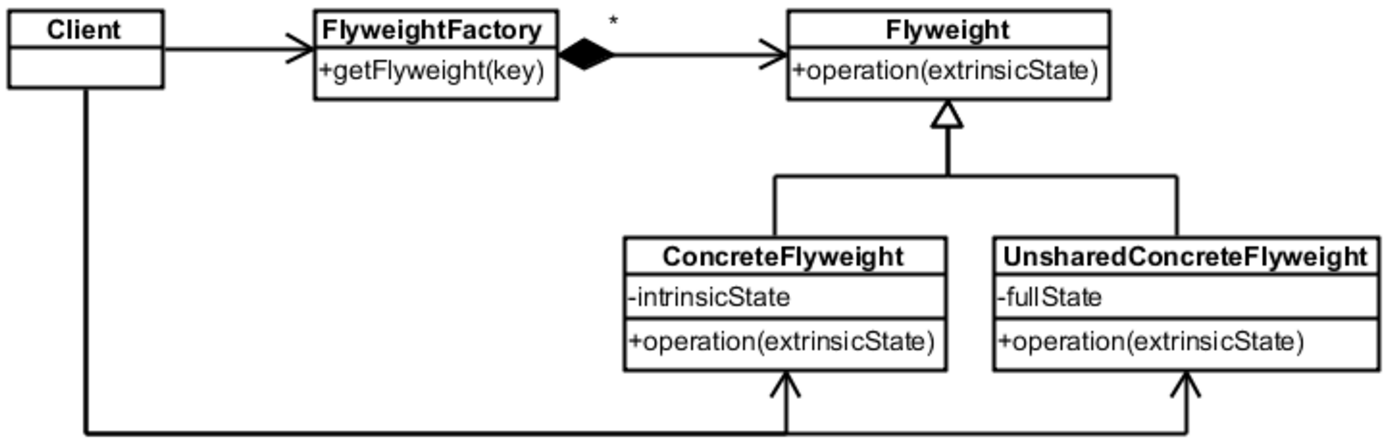
\includegraphics[width=0.85\textwidth]{flyweight.png}
\end{center}

Сами разделяемые объекты-приспособленцы (буквы в нашем примере) --- это наследники Flyweight, у которого есть операции, принимающие внешнее состояние. Приспособленцы могут иметь разделяемое внутреннее состояние (в случае с буквой это код символа, например), и, комбинируя внутреннее и внешнее состояние, выполнять операцию. Внешнее состояние хранится в клиенте, причём хранится как-то компактно. Клиент напрямую Flyweight-ы не создаёт, а получает их от FlyweightFactory, которая следит за временем их жизни, содержит в себе пул готовых приспособленцев и может создавать их по мере необходимости --- потому что одним Flyweight-ом может пользоваться несколько клиентов сразу. Хотя клиент вправе хранить ссылку на Flyweight, которым пользуется. Flyweight может и не иметь внешнего состояния и не быть разделяемым (UnsharedConcreteFlyweight на диаграмме), но участвовать в общей иерархии наследования для единообразности операций и участия в иерархических структурах типа паттерна <<Компоновщик>> (например, изображения в тексте, скорее всего, уникальны, но клиент может работать с ними через общий интерфейс). Такие объекты фабрика просто создаёт каждому клиенту свои, не пытаясь делать их разделяемыми.

Во время выполнения структура объектов может выглядеть вот так:

\begin{center}
    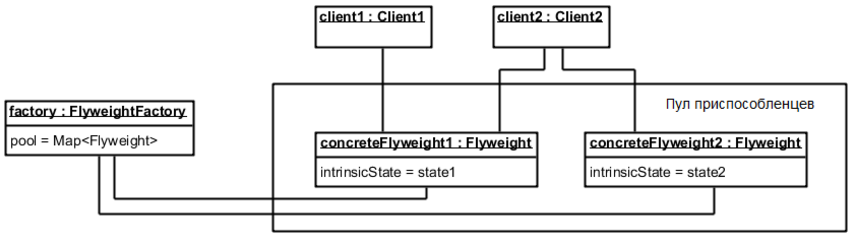
\includegraphics[width=0.9\textwidth]{flyweightObjects.png}
\end{center}

Фабрика содержит пул приспособленцев, клиенты ссылаются непосредственно на приспособленцев из пула, полученных через фабрику. При этом клиентов может быть несколько, и они могут быть никак не связаны друг с другом (даже не обязаны реализовывать общий интерфейс). Один приспособленец может разделяться между несколькими клиентами (каждый из которых хранит своё внешнее состояние для него), один клиент может пользоваться несколькими приспособленцами. Более того, один клиент может иметь несколько ссылок на одного и того же приспособленца (и передавать ему разные внешние состояния в зависимости от контекста). При этом клиенты должны получать приспособленцев через фабрику, но хранить ссылку на фабрику в процессе работы они не обязаны.

Паттерн довольно специфичен и редко встречается на практике, потому что для успешного применения надо, чтобы были выполнены все эти условия:

\begin{itemize}
    \item в приложении используется много мелких объектов, хранить каждый из которых отдельно дорого;
    \item эти объекты допускают содержательное разделение на внешнее и внутреннее состояние (даже модельный пример с текстовым редактором в этом плане не очень, потому что внутреннее состояние у букв очень уж жалкое, так что в реальной жизни стоило бы считать элементарным объектом не букву, а run);
    \item при этом внешнее состояние должно быть вычислимо или допускать ещё какой-то способ компактного хранения;
    \item при этом идентичность объектов должна быть не важна (то есть клиенты никогда не сравнивают их по ссылкам\footnote{В стандартной библиотеке Java в силу специфики реализации генериков есть так называемые обёрточные классы для элементарных типов, например, для типа int есть обёрточный класс Integer, представляющий полноценные объекты, лежащие на куче, с одним полем типа int. Создаются объекты обёрточных классов часто с помощью статического метода valueOf(), например, \mintinline{java}{Integer.valueOf(10)}. Ну и кому-то пришло в голову, что можно же первые 256 значений (от -128 до 127) создать заранее и возвращать всегда одни и те же, раз они часто используются, а остальные значения создавать по необходимости. А ещё в Java нет перегрузки операторов, поэтому == --- это всегда ссылочное сравнение. Поэтому, внезапно, \mintinline{java}{Integer.valueOf(10) == Integer.valueOf(10)}, но \mintinline{java}{Integer.valueOf(150) != Integer.valueOf(150)}. Сколько новичков вынесли с собеседования на этом вопросе...});
    \item в идеале приспособленцы должны обладать семантикой типов-значений;
    \item и главное, чтобы при применении паттерна был измеримый и ощутимый выигрыш, поскольку сложность кода паттерн увеличивает очень серьёзно, да и вероятность ошибок (особенно связанных со ссылочными сравнениями) возрастает значительно.
\end{itemize}

\subsection{Детали реализации}

Самое сложное в применении паттерна --- это разделение состояния на внутреннее и внешнее так, чтобы внутреннее состояние было разделяемым, а внешнее было вычислимым или позволяло себя эффективно хранить. Если различных внешних состояний столько же, сколько и исходных объектов, то смысла в применении паттерна никакого. Например, в текстовом редакторе <<run>> может хранить состояние для целого набора букв, так что там применение паттерна осмысленно.

Клиенты не могут создавать приспособленцев, а могут получать их только из фабрики (иначе трудно обеспечить разделение приспособленцев между клиентами). При этом стоит заранее подумать о механизме удаления неиспользуемых приспособленцев. Такой механизм вполне может и не понадобиться --- например, даже 110 тысяч <<букв>> алфавита Unicode ничего страшного с памятью не сделают, так что их можно просто создать заранее и хранить в пуле всё время работы приложения. При этом используются из них в одном документе не больше пары сотен, так что если мы сделаем фабрику, которая создаёт <<букву>> при необходимости и хранит её дальше до конца, это будет просто прекрасно. Однако если приспособленцев может быть много (например, разделяемые строки в механизме интернирования строк в компиляторе\footnote{Статья на Хабре про интернирование строк в C\#: \url{https://habr.com/ru/post/224281/} (дата обращения: 20.08.2021г)}), можно реализовать механизм удаления неиспользуемых приспособленцев (хотя конкретно компиляторы вряд ли удаляют что-то из пула интернирования, но не знаю). Для этого можно использовать что-то вроде подсчёта ссылок --- фабрика, выдавая приспособленца клиенту, запоминает, что клиент его взял, а как только приспособленец клиенту становится не нужен, он говорит фабрике, что его освободил, и если все клиенты освободили приспособленца, он удаляется.

Напомним, что приспособленцы по возможности должны обладать семантикой типов-значений, то есть операция сравнения у них проверяет равенство их атрибутов, а не ссылочное равенство (поскольку два объекта на самом деле могут быть одним и тем же объектом, либо просто случайно иметь одинаковые атрибуты --- системе должно быть без разницы). Заодно надо делать их немутабельными в плане внутреннего состояния, иначе если в одном клиенте что-то поменяют, это увидят все остальные клиенты, и в общем случае это плохая идея. Немутабельность включает в себя отсутствие ссылок на мутабельные объекты, даже если сами ссылки немутабельны --- например, предоставлять доступ к массиву во внутреннем состоянии приспособленца никому нельзя.Ещё часто забывают, что если мы переопределяем операцию сравнения (что нужно для семантики типа-значения), то надо не забыть и переопределить операцию получения хеш-кода --- если объекты равны, их хеш-коды обязаны совпадать (но не наоборот).

\end{document}
